Anstatt die einzelnen Iterationen der Funktionsmuster im Detail zu beschreiben, werden hier nur die herausragenden Eigenschaften der verschiedenen Iterationen dargestellt.  Dies soll einen Überblick über die Fortschritte und technischen Lösungen bieten, die im Laufe des Projekts entwickelt wurden. Die Eigenschaften werden teilweise in späteren Funktionsmustern nicht erneut umgesetzt wurden.


\textbf{Erste Iteration}

\begin{itemize}
    \item Eine neue Messung kann durchgeführt werden, indem das alte feuchte Tape mit einem wasserdichten Klebeband abgedeckt wird. Auf dieses trockene Klebeband wird manuell ein neues Tape aufgetragen.
    \item Die optische Auswertung kann mit einem Smartphone erfolgen, wodurch kein zusätzliches Material benötigt wird, da ein Smartphone bereits vorhanden ist.
\end{itemize}

\textbf{Zweite Iteration}

\begin{itemize}
    
    \item Das Tape wird auf einen Block aus extrudiertem Polystyrol (XPS) montiert, um den Einfluss eines warmen Tapehalters auf den Schnee zu reduzieren.
    \item Mit einem unter Druck stehenden inertem Gas wird der an den Tapes haftende Schnee abgeblasen.
    \item Die Lichtbox ist in zwei Kompartimente unterteilt: ein schwarzes, um Streulicht von außen zu minimieren, und ein helles, um das Licht der LED gleichmäßig auf die Tapes zu reflektieren.
    \item Die Tapehalter werden mit Elastomeren sicher an die Lichtbox angedrückt, was eine freie Rotation der Lichtbox ermöglicht.

\end{itemize}

\textbf{Dritte Iteration}

\begin{itemize}
    \item Die Gewichte haben Markierungen, die es ermöglichen, die Probe mit definierter kinetischer Energie auf den Schnee aufzubringen.
    \item Die Gewichte werden 20 cm oberhalb des Schwerpunkts von Kunststoffführungen gehalten, um ein Umkippen des Tapes während der Messung zu verhindern.
\end{itemize}

\textbf{Vierte Iteration}

\begin{itemize}
    \item Die Lichtbox kann zusammengefaltet werden, was einen platzsparenden Transport zur Versuchsort ermöglicht.
    \item Die Beleuchtung der Tapes in der Lichtbox erfolgt durch zwei LED-Panels und Diffusoren, die für eine gleichmäßige Ausleuchtung sorgen.
    \item Mit einem Kältemittel und einer Wärmebildkamera wird sichergestellt, dass die Tapes keine eigene Wärmeenergie besitzt, die den Schnee aufschmelzen könnte.
    \item Die Gewichte sind modular mit 36-g-Platten zusammengesetzt, was eine Anpassung an verschiedene Schneesorten ermöglicht.
\end{itemize}

\textbf{Fünfte Iteration}

\begin{itemize}
    \item Zur optischen Auswertung wird ein Raspberry Pi mit dem HQ-Kameramodul verwendet, was die Weiterverarbeitung der aufgenommenen Bilder erleichtert.
    \item Die Lichtbox ist in einer Kunststoffkiste untergebracht, um das Streulicht aus der Umgebung effektiv zu blockieren.
      \item Die Lichtbox ist auf der Innenseite mit einem schwarzen Samt Stoff ausgekleidet, um das Licht der LEDs besser zu kontrolieren.
\end{itemize}


\begin{figure}
    \centering
    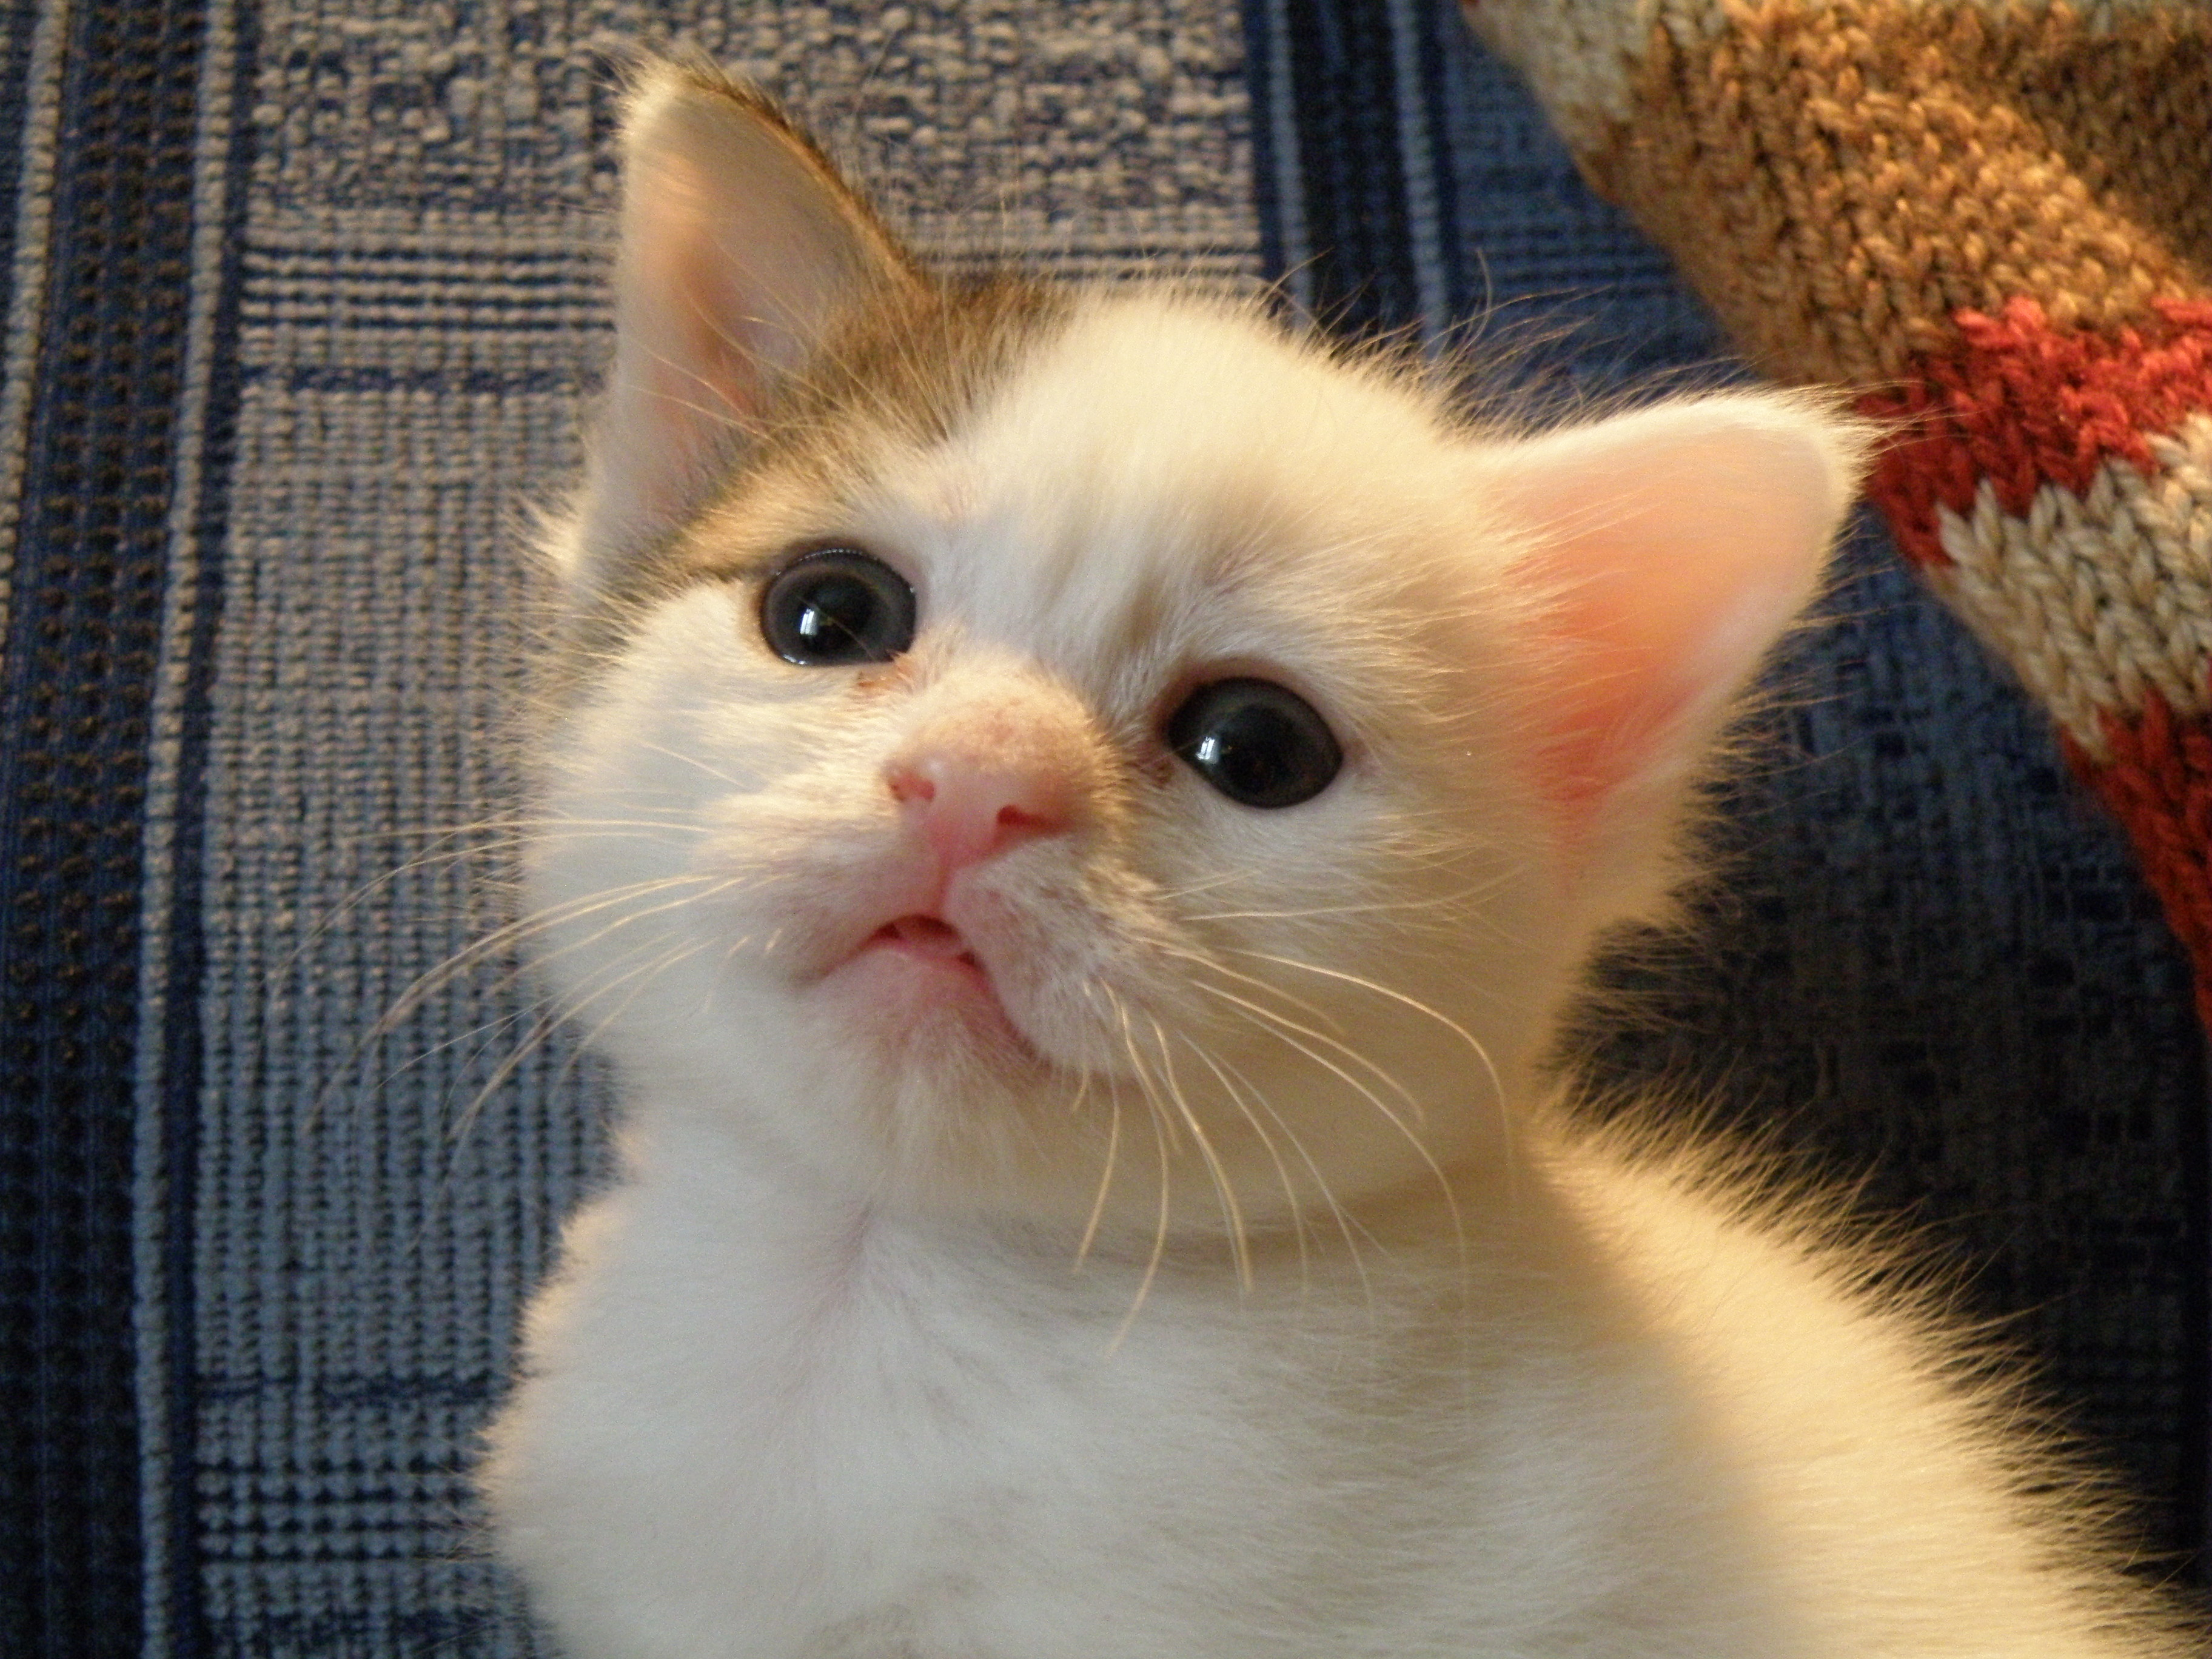
\includegraphics[width=0.8\textwidth]{Bilder/Photo_of_a_kitten.jpg}
    \caption{Fünfte Iteration}
    \label{fig:Peli}
\end{figure}
